\documentclass[a4paper,10pt,titlepage]{article}

\usepackage{geometry}
\usepackage{amsmath}
\usepackage{amssymb}
\usepackage{txfonts}
\usepackage{microtype}
\usepackage{epsfig}
\usepackage{graphicx}
\usepackage{moreverb}
\usepackage{hyperref}
\usepackage{listings}
\usepackage{xcolor}
\usepackage{textcomp}
\definecolor{listinggray}{gray}{0.98}
\definecolor{lbcolor}{rgb}{0.98,0.98,0.98}
\lstset{
	backgroundcolor=\color{lbcolor},
	tabsize=4,
	rulecolor=,
	language=matlab,
    basicstyle=\scriptsize\ttfamily,
    upquote=true,
    aboveskip={1.5\baselineskip},
    columns=fixed,
    showstringspaces=false,
    extendedchars=true,
    breaklines=true,
    prebreak = \raisebox{0ex}[0ex][0ex]{\ensuremath{\hookleftarrow}},
    frame=single,
    showtabs=false,
    showspaces=false,
    showstringspaces=false,
    identifierstyle=\ttfamily,
    keywordstyle=\color[rgb]{0,0,1},
    commentstyle=\color[rgb]{0.133,0.545,0.133},
    stringstyle=\color[rgb]{0.627,0.126,0.941},
}
\usepackage{eso-pic}
\usepackage{ifthen}

\AddToShipoutPictureBG{\ifthenelse{\equal{\value{page}}{0}}{}{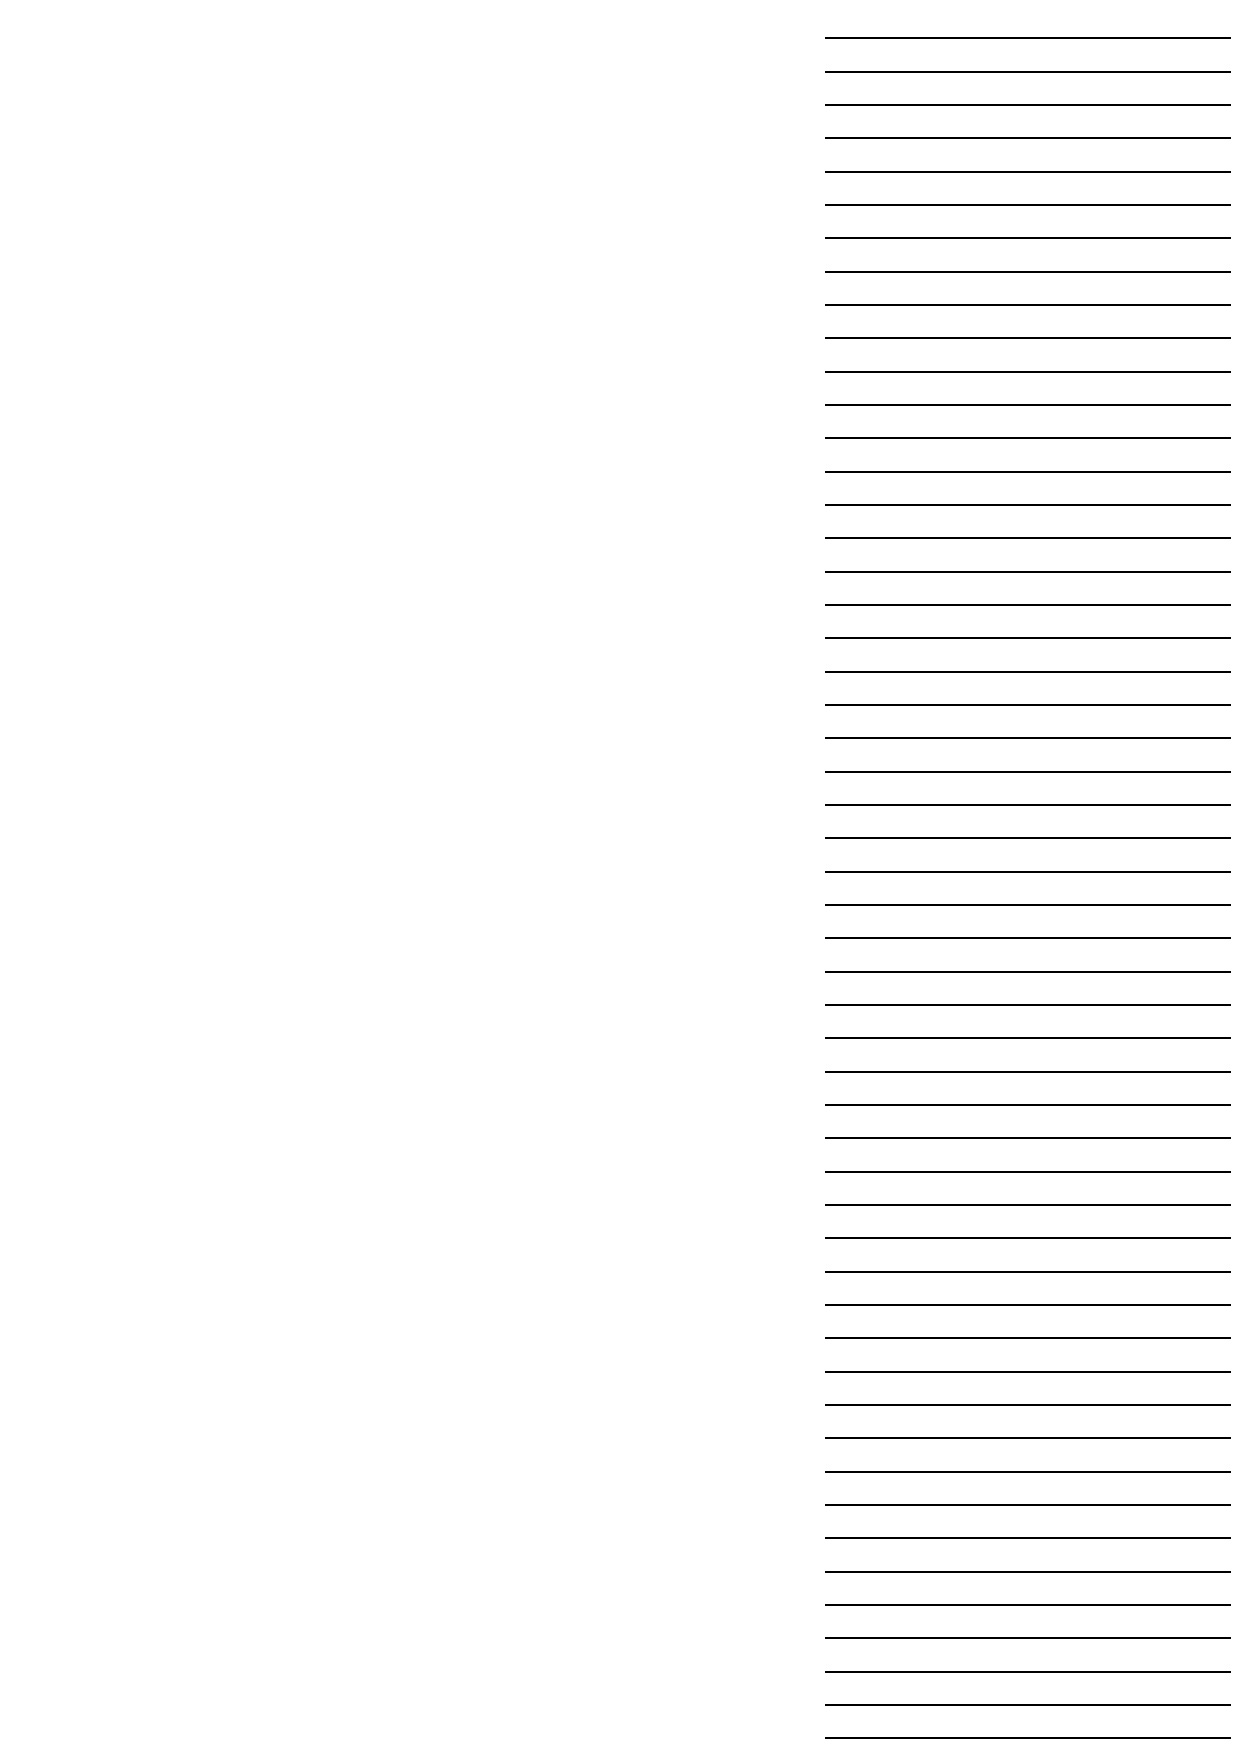
\includegraphics{template_files/backgroundlines}}}


\usepackage{tikz}
\usepackage{pgfplots}
\usepackage{tikzscale}
\usepackage{graphicx}
\usepackage{float}
\usepackage{subcaption}
\usepackage{comment}
\usepackage{units}
\usetikzlibrary{external}\tikzexternalize


\title{H1a: Molecular Dynamics simulation - static properties}
\author{Victor Nilsson and Simon Nilsson}
\date{\today}

\begin{document}

\newgeometry{top=2cm,bottom=2cm,left=2cm,right=2cm}

\begin{titlepage}

\setcounter{page}{0}

\begin{center}
{\huge \bf \color{red} NB: The graded, first version of the report must be
                           returned if you hand in a second time! } \\
\vspace{3cm}
\makeatletter
{ \huge \@title } \\
\vspace{1cm}
{ \Large \@author }\\
\vspace{1cm}
{ \Large \@date }\\
\makeatother
\end{center}

\vfill

\begin{flushright}
{\Large
\begin{tabular}{|c|c|c|}
\hline
Task N\textsuperscript{\underline{o}} & Points & Avail.\ points \\ \hline
\hspace{3cm} & \hspace{3cm} & \hspace{3cm} \\ \hline
~ & ~ & ~ \\ \hline
~ & ~ & ~ \\ \hline
~ & ~ & ~ \\ \hline
~ & ~ & ~ \\ \hline
~ & ~ & ~ \\ \hline
~ & ~ & ~ \\ \hline
~ & ~ & ~ \\ \hline
$\sum$ & ~ & ~ \\
\hline
\end{tabular}}
\end{flushright}

\end{titlepage}

\newgeometry{top=2cm,bottom=2cm,left=1.5cm,right=7.4cm}


\section*{Introduction}

Molecular dynamics is the movement of atoms and molecules. Such a system can be simulated and what is of interest is e.g. the trajectories of the atoms given specific surrounding parameters such as temperature, pressure, crystal formation etc. For this homeproblem we study the dynamics of aluminium atoms in a FCC crystal lattice.

For the homeproblems we simulate the dynamics of the aluminium atoms by approximating their interactions by their internal positions. At the start of each simulation the atoms are placed on a FCC lattice with lattice parameter $\unit[4.046]{\AA}$ \cite{al_wiki}. These atoms are initially displaced about $\unit[5]{\%}$ of the lattice spacing and their velocities are set to zero.

\section*{Problem 1}

\begin{figure}[H]
    \centering
    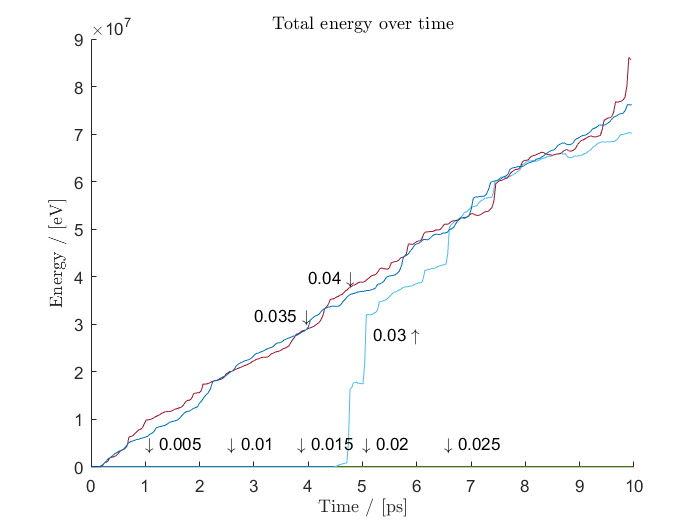
\includegraphics[width=\textwidth]{graphics/task1/energy.png}
    \caption{For different time-steps the energy evolves differently over time, in the figure we there are four simulations with different time-steps. The time-steps increases with $\unit[0.01]{ps}$ for each simulation and the total energy starts to increase for time-steps of $\unit[0.03]{ps}$.}
    \label{fig:timestep}
\end{figure}

For the simulations we updated the positions and velocities of the particles by applying the velocity verlet algorithm.

\begin{itemize}
\item $v \leftarrow v +\frac{1}{2}a\Delta t, \;$ update velocity from current acceleration.
\item $q \leftarrow q +v\Delta t, \;$ update displacement from current velocity.
\item $a \leftarrow a, \;$ update acceleration from the applied forces.
\item $v \leftarrow v +\frac{1}{2}a\Delta t, \;$ update velocity from new acceleration.
\end{itemize}

For this algorithm to be stable, we need to choose a time-step that conserves the total energy. With the algorithm implemented we can simulate the system and study the time evolution of the total energies. In Fig. \ref{fig:timestep} we can see the implications of different time-steps. We can see that the energy is unstable for $\Delta t = \unit[0.03]{ps}$ and stable for the previous one at $\Delta t = \unit[0.025]{ps}$. To have some safety margin we will, for the rest of the report, use a time-step of $\Delta t = \unit[0.005]{ps}$.

\section*{Problem 3}

\begin{figure}[H]
    \centering
    \captionsetup[subfigure]{justification=centering}
    \begin{subfigure}[b]{0.40\textwidth}
        \centering
        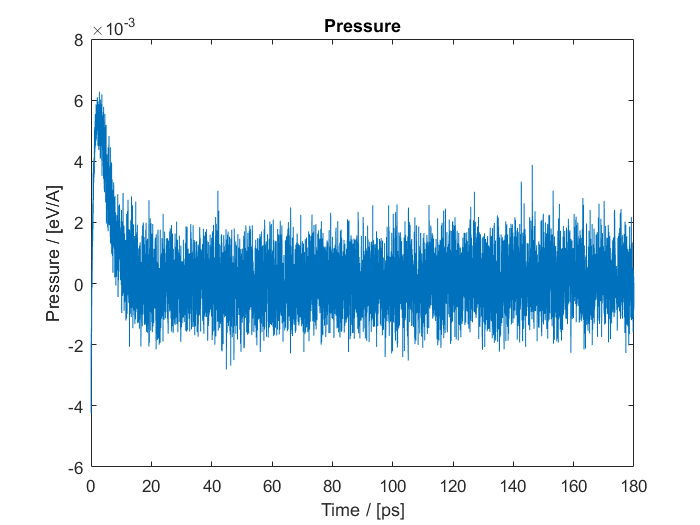
\includegraphics[width=\textwidth]{graphics/task3/pressure.png}
    \end{subfigure}
    \begin{subfigure}[b]{0.40\textwidth}
        \centering
        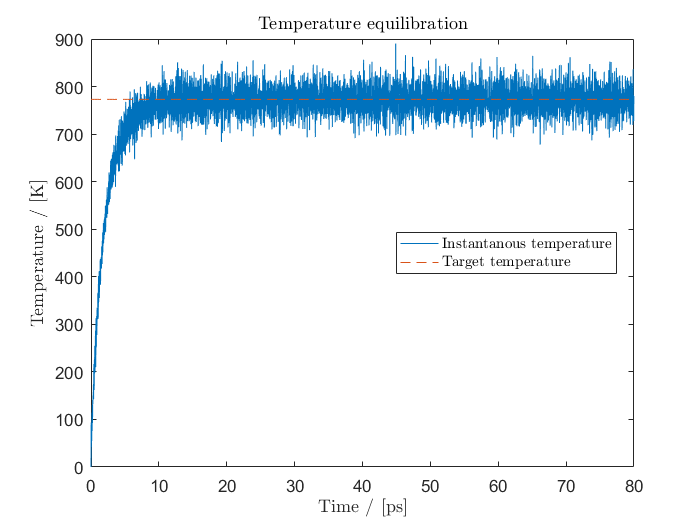
\includegraphics[width=\textwidth]{graphics/task3/temperature.png}
    \end{subfigure}
    \begin{subfigure}[b]{0.40\textwidth}
        \centering
        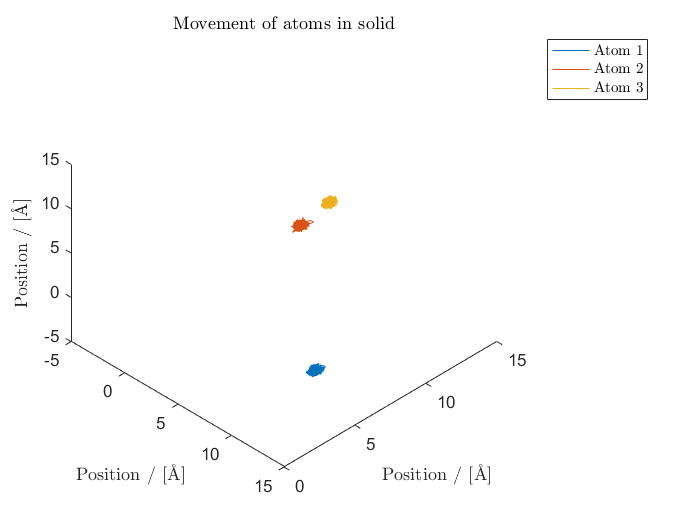
\includegraphics[width=\textwidth]{graphics/task3/traj.png}
    \end{subfigure}
    \caption{\textit{Upper left:} The time evolution of the pressure during equilibration. The target pressure was set to $\unit[1]{atm} = \unit[6.3249e^{-7}]{eV/\AA}$. \textit{Upper right:} The time evolution of the temperature during equilibration. The target temperature was set to 500$^\circ$ C and we can see that it quickly reaches the target temperature. \textit{Lower:} 3D plot of trajectories for three of the aluminium particles during 100 ps after the equilibration process. As we can see they stay close to the initial position, which indicates that the system is in its solid state. Note that the scales are not the same on all axes.}
    \label{fig:equilibrium500}
\end{figure}

The third problem was about implementing routines for equilibrating the molecular dynamics system to a specified temperature, $T_{eq} = 500^\circ$ C, at pressure $P_{eq} = 1$ atm. The equilibration was implemented using scaling of the velocities and the total volume, and consquently the positions of the molecules as well. The equations used can be found in appendix D in the molecular dynamics lecture notes \cite{lecnotes}. The goal was to study the temperature and pressure after the equilibration process through constant energy and volume simulation. We also plot the trajectories of a few particles to show that the system is still in a solid state (Fig. \ref{fig:equilibrium500}, lower subfigure).

The three main parameters for the equilibration are the timestep (used in the velocity Verlet algorithm) $\Delta t$ and the temperature and pressure relaxation times, $\tau_T$ and $\tau_P$ respectively. The timestep used was 5 fs and the temperature relaxation time was chosen to be $\tau_T = 100 \Delta t$, i.e. choosing the $\Delta t/\tau_T$ quotient in the $\alpha_T$ calculation to be equal 0.01.

When equilibrating the pressure the isothermic compressibility, $\kappa_T$, is used when computing $\alpha_P(t)$. The isothermic compressibility for aluminium is 0.01385 GPa$^{-1}$ \cite{knowledgedoor}, but $\tau_P$ is instead chosen in such a way thatv $\kappa_T$ is cancelled out. For these simulation we chose $\tau_P = 100\Delta t \kappa_T$.

% parameters: tau, delta t, kappa,

In order to set the system to a certain temperature, a technique involving scaling all the velocities during a equilibrating state. Since the temperature depends on the kinetic energies which in turn depends on the velocities, the  temperature can thusly be changed by changing velocities. In figure \ref{fig:equilibrium500} we can see the temperature after setting the temperature to $\unit[500]{C^\circ}$. There are some fluctuations in the beginning due to the rescaling of the velocities.


\section*{Problem 4}

\begin{figure}[H]
    \centering
    \captionsetup[subfigure]{justification=centering}
    \begin{subfigure}[b]{0.40\textwidth}
        \centering
        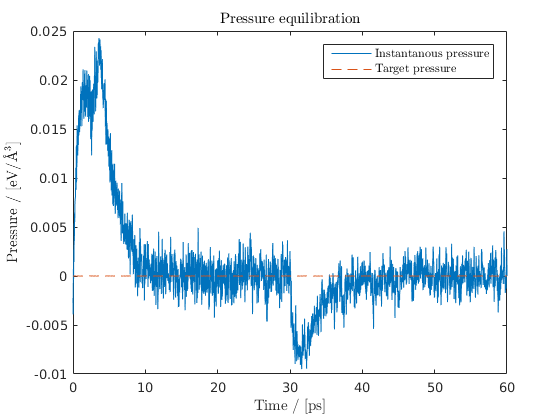
\includegraphics[width=\textwidth]{graphics/task4/pressure.png}
    \end{subfigure}
    %\begin{subfigure}[b]{0.40\textwidth}
    %    \centering
    %    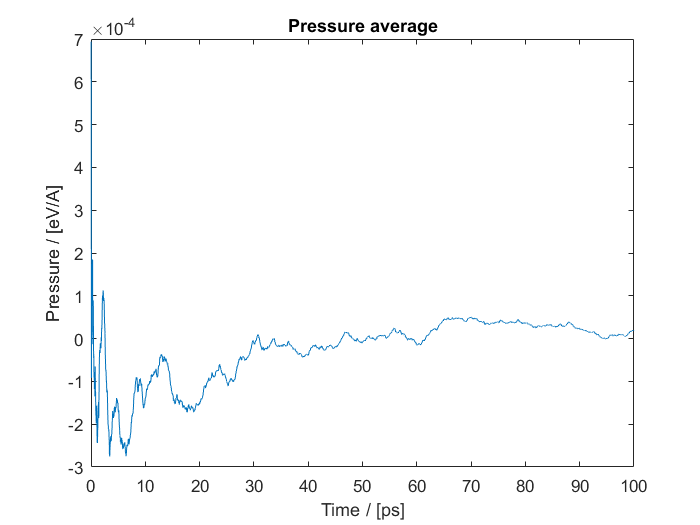
\includegraphics[width=\textwidth]{graphics/task4/pressure_avg.png}
    %\end{subfigure}
    \begin{subfigure}[b]{0.40\textwidth}
        \centering
        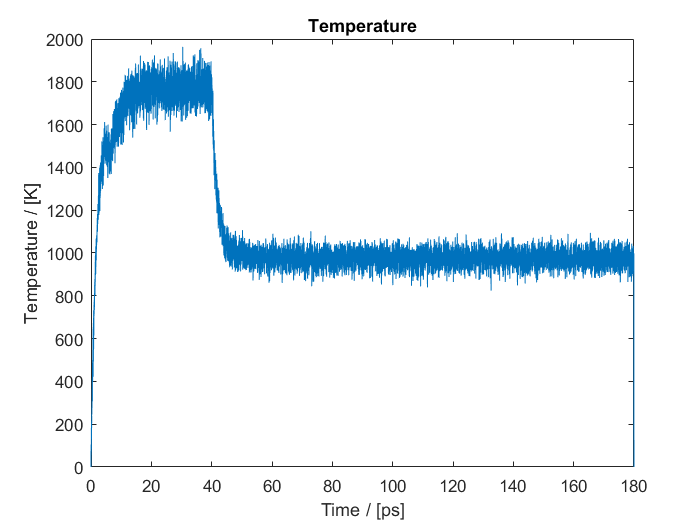
\includegraphics[width=\textwidth]{graphics/task4/temperature.png}
    \end{subfigure}
    %\begin{subfigure}[b]{0.40\textwidth}
    %    \centering
    %    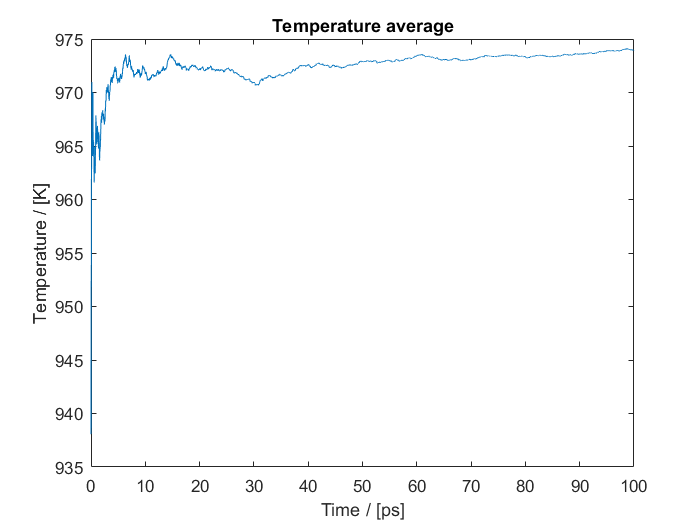
\includegraphics[width=\textwidth]{graphics/task4/temperature_avg.png}
    %\end{subfigure}
    \begin{subfigure}[b]{0.40\textwidth}
        \centering
        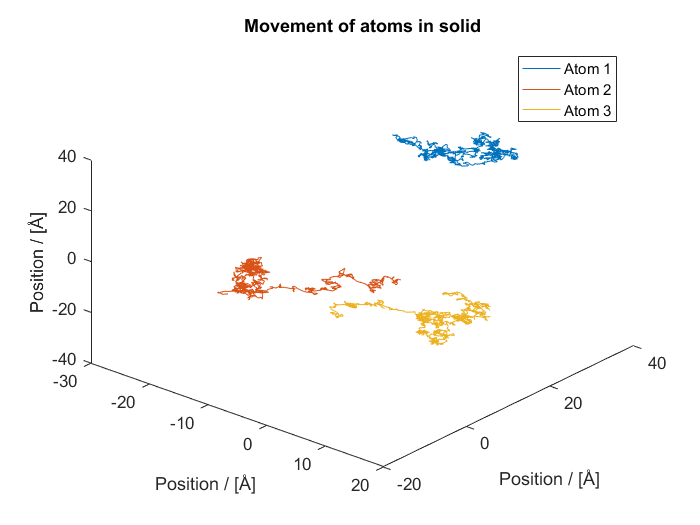
\includegraphics[width=\textwidth]{graphics/task4/traj.png}
    \end{subfigure}
    \caption{\textit{Upper left:} The time evolution of the pressure during equilibration. The sudden bump at 40 ps is because the target temperature is changed from 1 500$^\circ$ C to 700$^\circ$ C, causing rapid changes in the pressure. The first equilibration at a higher temperature is to ensure that the system enters its liquid state. \textit{Upper right:} The time evolution of the temperature during equilibration. \textit{Lower:} 3D plot showing the trajectories of three particles during 100 ps after the equilibration. As we can see they do not stay close to their initial position, which indicates that the system has melted.}
    \label{fig:equilibrium700}
\end{figure}

The fourth problem was very similar to the third one, with the exception that the system was to be equilibrated to a temperature of 700$^\circ$ C---which is higher than the melting point of aluminium (660$^\circ$ C \cite{al_wiki}). Effectively, what is done is that the system is melted. The target pressure was kept at 1 atm. Other parameters are also the same as in problem 3.

To ensure that the system would enter its melted state, at first, a target temperature of $1\,500^\circ$ C was set which was then lowered to 700$^\circ$ C. The switch can clearly be seen in both the pressure and temperature plots (upper left and right in Fig. \ref{fig:equilibrium700}).

Like in the previous problem, a few trajectories have been plotted (Fig. \ref{fig:equilibrium700}, lower). Unlike problem 3, we see that the particles do not remain close to their starting position for longer times, indicating that the system has indeed melted.

After equilibration to 700$^\circ$ C and 1 atm the average temperature obtained were approx. 714$^\circ$ C and $3.82 \cdot 10^{-4}$ eV/\r{A}$^3$. Similar to the third problem, the average pressure is much larger than intended, but we have not found a way of correcting it.

\section*{Problem 5}

\noindent One interesting thermal property of a material is the heat capacity. We can calculate it from fluctuations in either the kinetic or the potential energies, as
\begin{equation}
C_v=\frac{3Nk_B}{2}\left[1-\frac{2}{3Nk_b^2T^2}\left\langle \left(\delta \epsilon_{kin}\right)^2  \right\rangle_{NVE} \right]^{-1} \text{or}
\end{equation}

\begin{equation}
C_v=\frac{3Nk_B}{2}\left[1-\frac{2}{3Nk_b^2T^2}\left\langle \left(\delta \epsilon_{pot}\right)^2  \right\rangle_{NVE} \right]^{-1}.
\end{equation}

From our MD simulations we obtained the values found in {Table \ref{tab:prob5}} for $C_V$ when using the potential and kinetic energy fluctuations respectively. The same method and parameters as in problem 3 and 4 were used.

\begin{table}[h!]
	\centering
	\caption{Heat capacity obtained by measuring energy fluctuations in Problem 5.}
	\begin{tabular}{l|cc}
		\hline \textbf{Temperature} & \textbf{500$^\circ$ C} & \textbf{700$^\circ$ C} \\ \hline
		$C_V / (\unit{eV/kg\,K})$ (kinetic) & $4.9634 \cdot 10^{-2}$ & $6.7474 \cdot 10^{-2}$ \\
		$C_V / (\unit{eV/kg\,K})$ (potential) & $4.9686 \cdot 10^{-2}$ & $6.7579 \cdot 10^{-2}$ \\ \hline
	\end{tabular}
	\label{tab:prob5}
\end{table}

From experiments the heat capacity for aluminium in a solid is found to be $\unit[0.900]{J/g^\circ C}$ \cite{al_heat_solid} and for the liquid $\unit[1.18]{J/g^\circ C}$ \cite{al_heat_liquid}. The ratio of these are $1.18/0.9=1.3111$ which is almost the same ratio we found from our simulations,
$6.7474/4.963=1.3594$.



\section*{Problem 6}

When instead using the relation
\begin{equation}
	C_V = \left( \frac{\partial E}{\partial T} \right)_{N,V}
\end{equation}
to compute the heat capacity, and approximate it with a difference quota, we obtain the results found in the table below.

\begin{table}[h!]
	\centering	
	\caption{Heat capacity obtained by approximating the partial energy derivative with respect to the temperature.}
	\begin{tabular}{l|cc}
		\hline \textbf{Temperature} & \textbf{500$^\circ$ C} & \textbf{700$^\circ$ C} \\ \hline
		$C_V / (\unit{eV/kg\,K})$ & $7.0759 \cdot 10^{-2}$ & $7.0093 \cdot 10^{-2}$ \\ \hline
	\end{tabular}
	\label{tab:prob6}
\end{table}

If we compare these results to those from the previous problem we see that they are slightly larger and the result for 700 degrees deviates by a larger margin. It's possible that a longer equilibration time would yield a more stable temperature than was obtained now and therefore a more accurate heat capacity. A longer measuring time would also increase the accuracy of the result, as well as doing more simulations and averaging the different results. A $\Delta T$ of 5$^\circ$ C was used here, but further experiementing with this parameter could yield a better result as well.

\section*{Problem 7}

The radial distribution function obtained can be found in figure~\ref{fig:radial}. Using Matlab we find that the first peak is at the distance 2.85 \r{A}, which corresponds to the shortest distance in a fcc structure with the unit cell length of 4.046 \r{A}. This is the distance between one of the corner atoms and a face centered atom close to that corner, which is expected.

\begin{figure}[H]
\centering
\captionsetup[subfigure]{justification=centering}
\begin{subfigure}[b]{0.40\textwidth}
	\centering
	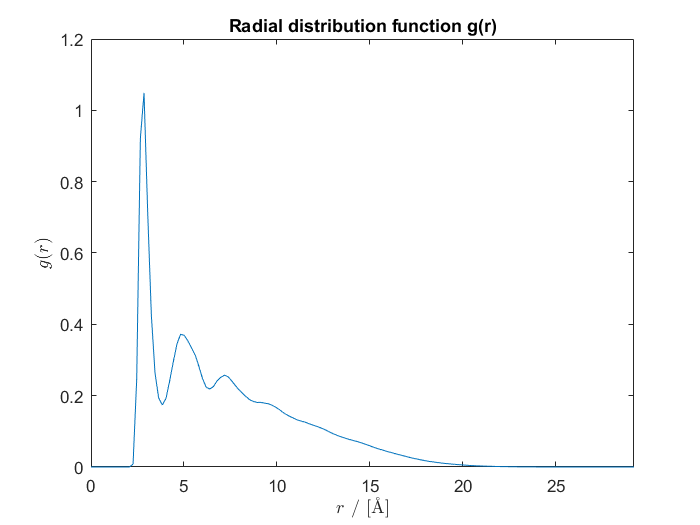
\includegraphics[width=\textwidth]{graphics/task7/radial.png}
\end{subfigure}
\caption{The radial function is computed by taking the histogram over all the internal distances between the atoms then divided by the random distribution of the same density.}
\label{fig:radial}
\end{figure}

Normally the radial distribution would converge to unity as the radius tends to infinity as over large distances the atoms are almost randomly distributed, this is not something we can see in out figure and is not expected. This is due to that our system is limited in size and we therefore can't find any particles for all distances as we have already counted that particle in the opposite direction.

With Matlab we find that the first local minimum is localized at $r_m = 3.7797$, giving us the coordination number $I(r_m) \approx 12.928$. The expected coordination number for an fcc structure is 12 \cite{al_coordination_nbr}, but our result is slightly higher. This is expected since the system is melted and the particles move around more freely. If the system was solid we would expect a result closer to 12.

\section*{Problem 8}

In Problem 8 we were, once again, tasked to examine the aluminium particles at 700$^\circ$ C and 1 atm. This time we examined the static structure factor $S(q)$ through 2 different methods; by integrating the result from the previous problem in accordance to Eq. (58) in \cite{lecnotes} and by simulating the system and evaluating Eq. (55) in \cite{lecnotes}.

Below (Fig.~\ref{fig:StaticStructure}) are two plots showing the approximations of the static structure function. The leftmost figure is obtained by integrating the result from Problem 7 and the rightmost one is obtained via simulation. 

\begin{figure}[H]
    \centering
    \captionsetup[subfigure]{justification=centering}
    \begin{subfigure}[b]{0.40\textwidth}
        \centering
        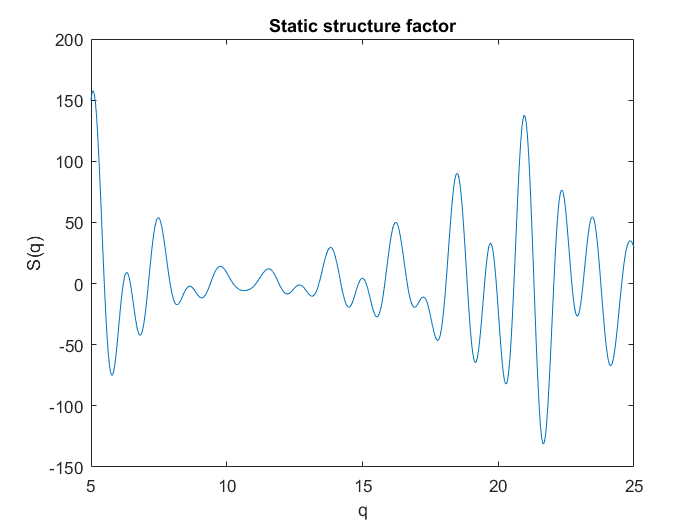
\includegraphics[width=\textwidth]{graphics/task8/integral.png}
    \end{subfigure}
    \begin{subfigure}[b]{0.40\textwidth}
        \centering
        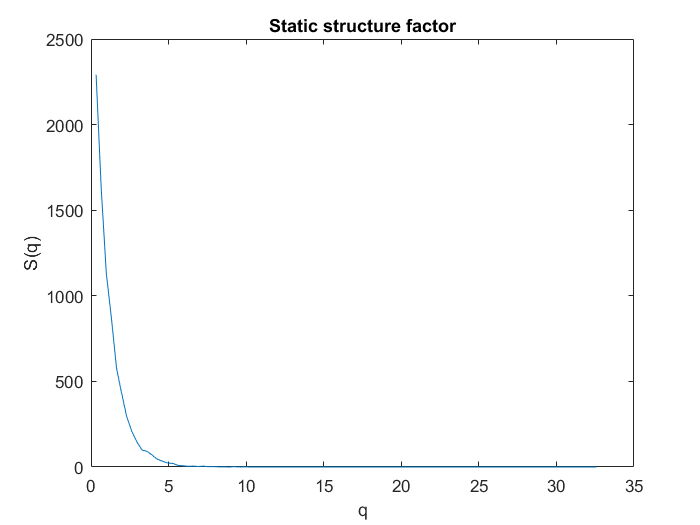
\includegraphics[width=\textwidth]{graphics/task8/simulated.png}
    \end{subfigure}
    \caption{The static structure function computed both from the radial distribution function in Figure \ref{fig:radial} (left) and using bins in Fourier space (right).}
    \label{fig:StaticStructure}
\end{figure}


\section*{Concluding discussion}


\vfill
\bibliography{references}
\bibliographystyle{plain} %TODO set bibstyle

\newpage
\appendix
\section{Source code}

\subsection{\texttt{Task1/MD\_main.c}}
\lstinputlisting[language=c, numbers=left]{../code/Task1/MD_main.c}

\subsection{\texttt{Task3/MD\_main.c}}
\lstinputlisting[language=c, numbers=left]{../code/Task3/MD_main.c}

\subsection{\texttt{Task4/MD\_main.c}}
\lstinputlisting[language=c, numbers=left]{../code/Task4/MD_main.c}

\subsection{\texttt{Task5/MD\_main.c}}
\lstinputlisting[language=c, numbers=left]{../code/Task5/MD_main.c}

\subsection{\texttt{Task6/MD\_main.c}}
\lstinputlisting[language=c, numbers=left]{../code/Task6/MD_main.c}

\subsection{\texttt{Task7/MD\_main.c}}
\lstinputlisting[language=c, numbers=left]{../code/Task7/MD_main.c}

\subsection{\texttt{Task8/MD\_main.c}}
\lstinputlisting[language=c, numbers=left]{../code/Task8/MD_main.c}
\lstinputlisting[language=c, numbers=left]{../code/Task8/alpotential.c}




\begin{comment}
\appendix

\section{Source Code}

Include all source code here in the appendix. Keep the code formatting clean,
use indentation, and comment your code to make it easy to understand. Also,
break lines that are too long. (Keep them under 80 characters!)

\subsection{Calculating pi using matlab: \texttt{pi.m}}
\lstinputlisting[language=matlab,numbers=left]{template_files/pi.m}

\subsection{Calculating pi using python: \texttt{pi.py}}
\lstinputlisting[language=python,numbers=left]{template_files/pi.py}

\subsection{Calculating pi using C: \texttt{pi.c}}
\lstinputlisting[language=c,numbers=left]{template_files/pi.c}

\end{comment}

\end{document}
